\newcommand{\checkbox}[1]{\item[$\square$]\textbf{#1}\\}

\chapter{Freshman checklist}

For a successful start to your studies, you should take care of a few organizational details in the first few weeks.
We have compiled the following checklist in descending order of priority.

\begin{itemize}

\checkbox{Apartment}
If you haven't found a place to stay yet, hurry up, because the best apartments are gone quickly.
If you would like to enjoy super-fast internet access
(provided by the \href{https://www.agdsn.de}{AG DSN}), we recommend the 
\href{https://www.studentenwerk-dresden.de/wohnen/wohnheimkatalog}{Studierendenwerk's dormitories}.
Alternatively, you can use portals like \href{https://wg-gesucht.de}{WG-Gesucht}.

\checkbox{Activate ZIH-Login}
All students receive a university account from the \textit{Zentrum für Informationsdienste und Hochleistungsrechnen} or ZIH in short.
This account is used for all important functions concerning your studies, be it wifi on campus or the registration for exams and courses.
You can also use it to access 
\href{https://tu-dresden.de/zih/dienste/service-katalog/arbeitsumgebung/zugang_datennetz/vpn}{the Uni-VPN}
(which you need, for example, to access old exams from home) and the
\href{https://tu-dresden.de/zih/dienste/service-katalog/zusammenarbeiten-und-forschen/datenaustausch/cloudstore}{Uni-Cloud}.

In order to use these services, it is necessary to activate your ZIH login with the IDM coupon in the 
\href{https://idm-coupon.tu-dresden.de}{Identity Manager}.
The coupon should have been delivered to your email address provided in the applicant portal.

\checkbox{Email}
You will receive an address of the form 
\textit{vona123a@msx.tu-dresden.de}
together with an alias 
\textit{firstname.lastname@mailbox.tu-dresden.de} from ZIH.
% Ältere Jahrgänge haben E-Mail-Adressen der Form
% \textit{s1234567\allowbreak{}@mail.zih.tu-dresden.de}, wundere dich also nicht,
% wenn du die noch siehst.
If your name already exists at the TU Dresden, 
the alias address for John Doe will be e.g. 
\textit{john.doe1@mailbox.tu-dresden.de}. 

You can access your mailbox via webmail and IMAP\@. 
Alternatively, you can set up a forwarding to a personal address. 
Many e-mails from the university are sent to these addresses. 
Therefore, make sure that you check your mail regularly or forward it to another address.
The ZIH has 
\href{https://tu-dresden.de/zih/dienste/service-katalog/arbeitsumgebung/e_mail/}{more information on e-mails}.

\checkbox{BAföG application}
You can find the application forms on the \href{https://www.bafög.de/de/alle-antragsformulare-432.php}{BMBF website}.
For further information, please contact the service office or your student services officer.
Don't put off applying too long, as your entitlement will not be valid until the month of application at the earliest.
Information about office hours at the Studierendenwerk can be found \href{https://www.studentenwerk-dresden.de/finanzierung/servicebuero.html}{here}.

\label{sec:ummelden}
\checkbox{Registering your residence}
Officially, you have to register your apartment within two weeks at the 
\href{https://www.dresden.de/de/rathaus/dienstleistungen/wohnsitz_meldung_d115.php}{responsible local office}.
If you register your apartment as a secondary residence, you will have to pay a tax on secondary residences.
This amounts to 10\% of the net rent per month.
You can find more information about this 
\href{https://www.stura.tu-dresden.de/zweitwohnungssteuer}{on the pages of the StuRa} or the 
\href{https://www.dresden.de/de/rathaus/dienstleistungen/zweitwohnungssteuer.php}{city of Dresden}.
Please do not forget that every household (shared flats can be combined!) has to pay the Rundfunkbeitrag.
So register or submit your BAföG exemption.

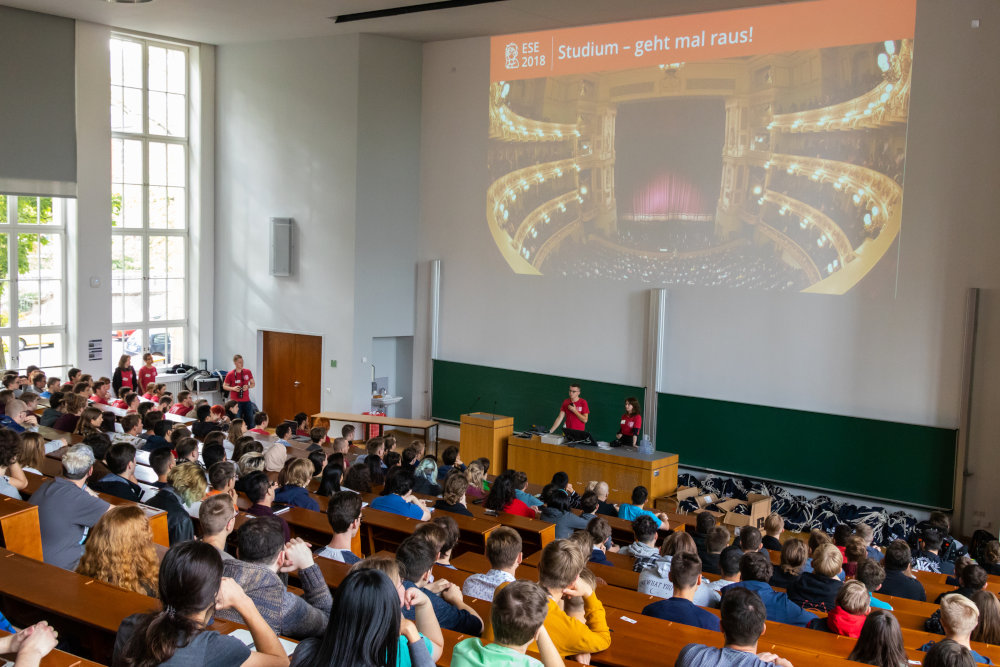
\includegraphics[width=.93\linewidth]{img/begruessung1.jpg}

\checkbox{Emeal card}
The Mensakarte allows you to pay cashless in the different refectories of the university.
You can get it during the ESE or in the refectories themselves for a deposit of 5\euro\ and by presenting the Emeal certificate, which you will find on your Semesterbogen.


\checkbox{WIFI}
You can access the internet with your devices both on campus and in the faculty premises. 
The network is called \textit{eduroam} and offers you secure internet access not only at the TU Dresden but also at many other universities worldwide. 
You get access with your ZIH login, here in the form 
   \textit{vona123a@tu-dresden.de}, 
and your password. For mobile devices like your smartphone 
\href{https://tu-dresden.de/zih/dienste/service-katalog/arbeitsumgebung/zugang_datennetz/wlan-eduroam}{%
ZIH recommends the setup via eduroam CAT}. 

\checkbox{Programming courses}
Especially for those without programming experience, the programming courses offered in the winter semester are highly recommended. 
Especially the C, Python and Java courses are very helpful to get through the first semesters. 
The courses usually take place during the week.
For details, refer to \href{mailto:programmierung@ifsr.de}{programmierung@ifsr.de} and keep an eye on the news on the \href{https://www.ifsr.de}{FSR page}.
You can also use the LinkedIn Learning courses that are accessible \href{https://www.slub-dresden.de}{through the SLUB}.

\label{sec:sprache}
\checkbox{(optional) Language courses}
TU Dresden offers language courses for English and many other languages. 
Enrollment for the language courses will be unlocked during the first two weeks of your studies, depending on the course. Check the 
\href{https://lskonline.tu-dresden.de/}{LSK pages} 
early to find out when this is. Most courses fill up very quickly.

\label{sec:sport}
\checkbox{(optional) Sports courses}
As with the language courses, it's first come, first served\ldots{} 
You can check the offer at the 
\href{https://tu-dresden.de/usz}{Universitätssportzentrum (USZ)}.
Once you have decided on a course and registered for it, all you have to do is print out the registration certificate and transfer the fee to the USZ bank account within three days.

\checkbox{Documents relevant to your studies}
The \href{https://tu-dresden.de/ing/informatik/studium/lehre}{Vorlesungsverzeichnis} and 
\href{https://tu-dresden.de/ing/informatik/studium/studienangebot}{the Prüfungs- und Studienordnung} can be found on the pages of the faculty.
Printed regulations are available at the FSR, but are also distributed during the seminar group meetings.
All important information about the individual lectures can be found on the respective pages of the institutes on the net.
The professors will tell you everything in the first lectures. 
Otherwise, a look at the \href{FSR page}{https://www.ifsr.de} might help you.

% TODO Wohnsitznachweis nach wie vor benötigt?
% (https://www.slub-dresden.de/service/benutzungsordnung/)
\checkbox{Library card}
You can get your library card at the counter of the SLUB (Zellescher Weg 18) after registering online and presenting your proof of residence, i.e. your identity card after you have changed 
\href{https://www.slub-dresden.de/besuchen/nutzerin-der-slub-werden}{your registration}.
Registration and borrowing of media is free of charge -- provided that you do not exceed the loan periods ;).

\checkbox{(optional) Visit FSR meetings}
\hyperlink{sec:fachschaftsrat}{Here}
 you can find more information about the FSR.

\checkbox{Fachschaftsrat elections}
Vote for your student representatives in the FSR Computer Science. Elections are held at the end of the year. 
Go vote! And even better: Get elected!


\checkbox{Exam enrollment}
From the beginning of next year you can register for exams in \href{https://jexam.inf.tu-dresden.de/}{jExam}.
The date will be announced on the page of the Prüfungsamt.
Register in time, otherwise you will not be able to take the exam.
Enroll in the exams of the subjects you have attended. Note that the first exam in math is already at the beginning of December. Good luck!

\checkbox{Re-registration for the summer semester}
From mid-January 2022 you can transfer the semester fee for the next semester.
You can find the exact amount and dates online \href{https://tu-dresden.de/imma/rueckmeldung}{here}.
Take care of it in time, otherwise you will be automatically exmatriculated!

\end{itemize}


\begin{figure}[h!]
\centering
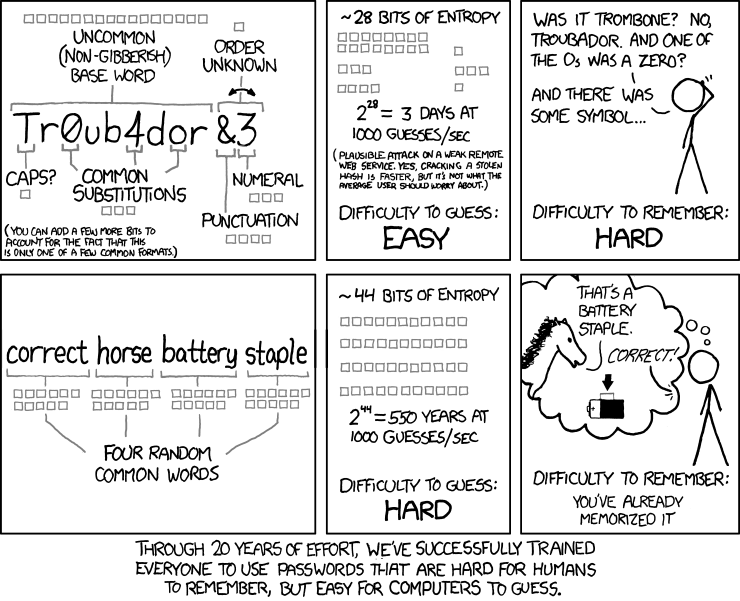
\includegraphics[width=.8\linewidth,keepaspectratio]{img/xkcd/password_strength.png}
\caption*{{\small
    \foreignlanguage{english}{
      \textit{To anyone who understands information theory and security and is in an infuriating argument with someone who does not (possibly involving mixed case), I sincerely apologize.\\\hspace*{1mm}\hfill(https://xkcd.com/936)}
    }
%     \foreignlanguage{english}{
%       \textit{\enquote*{Are you stealing those LCDs?} \enquote*{Yeah, but I'm doing it while my code compiles.}\\\hspace*{1mm}\hfill(https://xkcd.com/303)}
%     }
  }
}
\end{figure}
